\begin{exercise}
	Δίνεται κύκλος με κέντρο $Κ(7,7)$ και ακτίνα $r = 10$. 
	\begin{itemize}
	  \item Ποιό είναι το πρώτο pixel που θα φωτίσει ο αλγόριθμός σχεδιασμού κύκλου του Bresenham για το $2$ο οκταμόριο;
	  \item Ποια είναι τα $2$ αμέσως επόμενα pixel που θα φωτίσει ο αλγόριθμός σχεδιασμού κύκλου του Bresenham για το $2$ο οκταμόριο;
	  \item Να υπολογίστε  τα pixels που θα φωτισθούν από την εφαρμογή της συμμετρίας των $8$ δρόμων.
	\end{itemize}
\end{exercise}


\begin{solution}
	

\begin{lstlisting}[caption={Αλγόριθμος του Bresenham για σχεδιασμό κύκλου}]
function brescircle(xc, yc, r)
    # (xc, yc) are the coordinates of the circle's centre
    # r is the radius of the circle
    x = 0 
    y = r
    error = 3 - 2 * r
    
    while x <= y
        plot(x+xc, y+yc, 0)
        plot(x+xc, -y+yc, 0) 
        plot(-x+xc, y+yc, 0) 
        plot(-x+xc, -y+yc, 0) 
        plot(y+xc, x+yc, 0) 
        plot(-y+xc, x+yc, 0)
        plot(y+xc, -x+yc, 0) 
        plot(-y+xc, -x+yc, 0) 
        x = x + 1
        if error > 0
            y = y - 1
            error = error - 4*y
        end
        error = error + 4*x + 2
    end
end
\end{lstlisting}


Για τον κύκλο με κέντρο \( K(7, 7) \) και ακτίνα \( r = 10 \), θα έχουμε:

\begin{itemize}[noitemsep, topsep=0pt] % Reduce vertical spacing
\begin{multicols}{2} % Split into 2 columns
  \item \( x = 0 \)
  \item \( y = 10 \)
  \item \( error = 3 - 2 \cdot r = 3 - 20 = -17 \)
\end{multicols}
\end{itemize}


\begin{itemize}
  \item \underline{1η επανάληψη}
\lstset{style=tt}
		\begin{lstlisting}
		x == 0 $<=$ 10 $\Rightarrow$
			plot(7, 17) % (x+xc, y+yc)
			plot(7, -3)  % (x+xc, -y+yc)
			plot(-7, 17) % (-x+xc, y+yc)
			plot(-7, -3) % (-x+xc, -y+yc)
			plot(17, 7)  % (y+xc, x+yc)
			plot(-17, 7) % (-y+xc, x+yc)
			plot(17, -7) % (y+xc, -x+yc)
			plot(-17, -7) % (-y+xc, -x+yc)
			x = 1 %(x == x + 1)
			error == -17 $<$ 0 
				error = -17 + 4*1 + 2 = -11 %(error == error + 4*x + 2)
		\end{lstlisting}

  \item \underline{2η επανάληψη}

		\begin{lstlisting}
		x == 1 $<=$ 10 $\Rightarrow$
			plot(8, 17) % (x+xc, y+yc)
			plot(8, -3)  % (x+xc, -y+yc)
			plot(-8, 17) % (-x+xc, y+yc)
			plot(-8, -3) % (-x+xc, -y+yc)
			plot(17, 8)  % (y+xc, x+yc)
			plot(-17, 8) % (-y+xc, x+yc)
			plot(17, -8) % (y+xc, -x+yc)
			plot(-17, -8) % (-y+xc, -x+yc)
			x = 2 %(x == x + 1)
			error == -11 $<$ 0 
				error = -11 + 4*2 + 2 = -1 %(error == error + 4*x + 2)
		\end{lstlisting}

  \item \underline{3η επανάληψη}

		\begin{lstlisting}
		x == 2 $<=$ 10 $\Rightarrow$
			plot(9, 17) % (x+xc, y+yc)
			plot(9, -3)  % (x+xc, -y+yc)
			plot(-9, 17) % (-x+xc, y+yc)
			plot(-9, -3) % (-x+xc, -y+yc)
			plot(17, 9)  % (y+xc, x+yc)
			plot(-17, 9) % (-y+xc, x+yc)
			plot(17, -9) % (y+xc, -x+yc)
			plot(-17, -9) % (-y+xc, -x+yc)
			x = 3 %(x == x + 1)
			error == -1 $<$ 0 
				error = -1 + 4*3 + 2 = 13 %(error == error + 4*x + 2)
		\end{lstlisting}
\end{itemize}

\begin{figure}[hbt]
  \begin{center}
	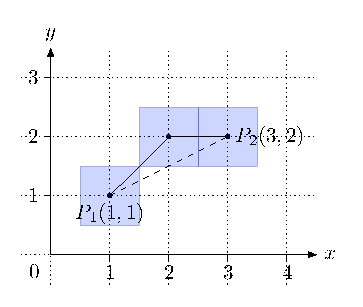
\includegraphics[scale=0.6]{Chapter1/Exercises/ex15/graph1.pdf}
  \end{center}
  \caption{Παράσταση πρώτων $3$ επαναλήψεων αλγορίθμου Bresenham για κύκλο κέντρου $Κ(7,7)$ και ακτίνας $r = 10$. Τα χρώματα για την $1$η, $2$η και $3$η επανάληψη είναι μπλε και πορτοκαλί αντίστοιχα. }
\end{figure}

\end{solution}